%%%%%%%%%%%%%%%%%%%%%%%%%%%%%%%%%%%%%%%%%%%%%%%%%%%%%%%%%%%%
%%  This Beamer template was created by Cameron Bracken.
%%  Anyone can freely use or modify it for any purpose
%%  without attribution.
%%
%%  The current presentation created by Jeferson L. R. Souza (jefecomp) is based on the template created by Cameron Bracken. 
%%  
%%  Small modifications have been introduced and anyone is free to use such modified version.
%%
%% Last Modified: June 14, 2015.

\documentclass[xcolor=x11names,compress]{beamer}

%% General document %%%%%%%%%%%%%%%%%%%%%%%%%%%%%%%%%%
\usepackage{graphicx}
\usepackage{tikz}
\usetikzlibrary{decorations.fractals}
%%%%%%%%%%%%%%%%%%%%%%%%%%%%%%%%%%%%%%%%%%%%%%%%%%%%%%


%% Beamer Layout %%%%%%%%%%%%%%%%%%%%%%%%%%%%%%%%%%
\useoutertheme[subsection=false,shadow]{miniframes}
\useinnertheme{default}
\usefonttheme{serif}
\usepackage{palatino}

\setbeamerfont{title like}{shape=\scshape}
\setbeamerfont{frametitle}{shape=\scshape}

\setbeamercolor*{lower separation line head}{bg=DeepSkyBlue4} 
\setbeamercolor*{normal text}{fg=black,bg=white} 
\setbeamercolor*{alerted text}{fg=red} 
\setbeamercolor*{example text}{fg=black} 
\setbeamercolor*{structure}{fg=black} 
 
\setbeamercolor*{palette tertiary}{fg=black,bg=black!10} 
\setbeamercolor*{palette quaternary}{fg=black,bg=black!10} 

\renewcommand{\(}{\begin{columns}}
\renewcommand{\)}{\end{columns}}
\newcommand{\<}[1]{\begin{column}{#1}}
\renewcommand{\>}{\end{column}}
%%%%%%%%%%%%%%%%%%%%%%%%%%%%%%%%%%%%%%%%%%%%%%%%%%

%%  user definitions and package declaration

%%  changing footer template
\setbeamertemplate{footline}[frame number] 
\setbeamertemplate{blocks}[rounded] [shadow=true]

%%  declaring picture extensions and default path
\DeclareGraphicsExtensions{.png, .jpg, .pdf}
\graphicspath{{pictures/}}

%% Supporting source code lists
\usepackage{listings}
\lstset{breakatwhitespace,
language=Java,
columns=fullflexible,
keepspaces,
breaklines,
tabsize=3, 
showstringspaces=false,
extendedchars=true}

%Text position
\usepackage{textpos}
\setlength{\TPHorizModule}{128mm}
\setlength{\TPVertModule}{96mm}

\usepackage{array}


%Puting text and other float elements over pictures
\usepackage[percent]{overpic}


%% Hyperlinks over all the document
\usepackage{hyperref}

%% Controlling text alignment
\usepackage{ragged2e}

%% Framed text
\usepackage{framed}

%% Math packages
\usepackage{amsmath}

\begin{document}

\title{Java Persistence API \\[4mm]

\includegraphics[keepaspectratio,width=.3\textwidth]{JPA}}
\subtitle{A Short Course \\ (Part I) \vspace*{-4mm}}
\author[Jeferson L. R. Souza (jefecomp) - All rights reserved.]{
	\textcolor{blue}{Jeferson L. R. Souza (jefecomp)} \\[1mm] 
	\textcolor{blue}{\textit{{\footnotesize PhD candidate / IT Consultant}}}\\[1.5mm]
	 \underline{{\footnotesize jefersonsouza@boldint.com}}
	 \vspace*{-6mm}
}
\date{{\footnotesize June 15, 2015}}


%%%%%%%%%%%%%%%%%%%%%%%%%%%%%%%%%%%%%%%%%%%%%%%%%%%%%%
%%%%%%%%%%%%%%%%%%%%%%%%%%%%%%%%%%%%%%%%%%%%%%%%%%%%%%
\begin{frame}[plain,noframenumbering]
\titlepage
\end{frame}

%%%%%%%%%%%%%%%%%%%%%%%%%%%%%%%%%%%%%%%%%%%%%%%%%%%%%%
%%%%%%%%%%%%%%%%%%%%%%%%%%%%%%%%%%%%%%%%%%%%%%%%%%%%%%
\section{\scshape JPA Design}
\subsection{What is the Java Persistence API?}
\begin{frame}{\underline{What is the Java Persistence API?}}
\begin{itemize}
\itemsep 12pt
\justifying
\item The Java Persistence API (JPA) is a specification defining a standard way to persist objects on storage systems;

\item The JPA itself is part of the Enterprise Java Beans (EJBs) 3.0 specification, which is defined in the JSR 220 (\url{https://jcp.org/en/jsr/detail?id=220});

\item In theory, the storage system utilised to persist objects of Java applications can be anything. However, JPA has been initially designed to allow saving and querying Plain Old Java Objects (POJOs) on relational databases such as MySQL, PostgreSQL, Oracle, etc;

\end{itemize}
\end{frame}

%%%%%%%%%%%%%%%%%%%%%%%%%%%%%%%%%%%%%%%%%%%%%%%%%%%%%%
%%%%%%%%%%%%%%%%%%%%%%%%%%%%%%%%%%%%%%%%%%%%%%%%%%%%%%
\subsection{JPA features}
\begin{frame}{\underline{JPA Features}}

\begin{itemize}
\itemsep 12pt
\justifying

 \item Object-oriented data and persistence model; 

\item Rich Metadata annotations for definition of persistence entities;

\item Object and query-level caching support;

\item Transactional object model support;

\item Enable on both JavaEE and JavaSE applications.

\end{itemize}

\end{frame}

%%%%%%%%%%%%%%%%%%%%%%%%%%%%%%%%%%%%%%%%%%%%%%%%%%%%%%
%%%%%%%%%%%%%%%%%%%%%%%%%%%%%%%%%%%%%%%%%%%%%%%%%%%%%%
\section{JPA Architecture}
\subsection{Main Components}
\begin{frame}{\underline{Main Components}}

\begin{center}
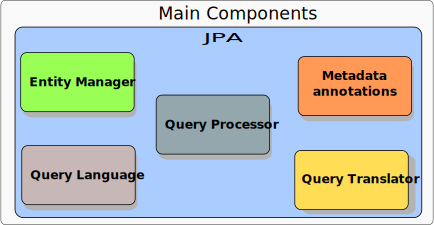
\includegraphics[keepaspectratio,width=.8\textwidth]{JPA-mainComponents}

The main abstract components of the Java Persistence API.
\end{center}
\end{frame}

%%%%%%%%%%%%%%%%%%%%%%%%%%%%%%%%%%%%%%%%%%%%%%%%%%%%%%
%%%%%%%%%%%%%%%%%%%%%%%%%%%%%%%%%%%%%%%%%%%%%%%%%%%%%%
\subsubsection{Entity Manager}
\begin{frame}{\underline{Entity Manager}}

\begin{itemize}
\itemsep 12pt
\justifying

\item Responsible to manager the life cycle of persistence entities within a domain dubbed Persistence Context;

\item Exposed interface with operations for save, delete, update, and query of entities on a storage system;

\item Internal characteristics and behaviour depends on JPA implementations;
\end{itemize}
\end{frame}
%%%%%%%%%%%%%%%%%%%%%%%%%%%%%%%%%%%%%%%%%%%%%%%%%%%%%%
%%%%%%%%%%%%%%%%%%%%%%%%%%%%%%%%%%%%%%%%%%%%%%%%%%%%%%
\subsubsection{Entity Manager}
\begin{frame}{\underline{Entity Manager} (1)}

{\footnotesize

\textcolor{red}{public interface} EntityManager \{ \\[2mm]

\textcolor{red}{public void} persist(Object entity); \\[2mm]

\textcolor{red}{public} $<$T$>$ merge (T entity); \\[2mm]

\textcolor{red}{public void} remove (Object entity); \\[2mm]

\textcolor{red}{public} $<$T$>$ find (Class$<$T$>$ entityClass, Object primaryKey); \\[2mm]

\textcolor{red}{public} $<$T$>$ getReference (Class$<$T$>$ entityClass, Object primaryKey); \\[2mm]

\textcolor{red}{public void} flush(); \\
\begin{center}
. \\
. \\
. \\
\end{center}
\}
}
\end{frame}


%%%%%%%%%%%%%%%%%%%%%%%%%%%%%%%%%%%%%%%%%%%%%%%%%%%%%%
%%%%%%%%%%%%%%%%%%%%%%%%%%%%%%%%%%%%%%%%%%%%%%%%%%%%%%
\subsubsection{Metadata Annotations}
\begin{frame}{\underline{Metadata Annotations}}

\begin{itemize}
\itemsep 12pt
\justifying

\item The way a POJO is identified as a persistence entity by JPA;

\item Types of annotations:

\begin{itemize}
\itemsep 12pt
\justifying

\item Entity Definition and Inheritance (\textcolor{red}{\textit{@Entity, @MappedSuperClass,} \ldots});

\item Entity Relations (\textcolor{red}{\textit{@OneToOne, @OneToMany, @ManyToOne, @MaToMany}});

\item Object Relational Mapping (\textcolor{red}{\textit{@Id, @Table, @Column, @JoinColumn,} \ldots}).
\end{itemize}
\end{itemize}
\end{frame}

%%%%%%%%%%%%%%%%%%%%%%%%%%%%%%%%%%%%%%%%%%%%%%%%%%%%%%
%%%%%%%%%%%%%%%%%%%%%%%%%%%%%%%%%%%%%%%%%%%%%%%%%%%%%%
\subsubsection{Metadata Annotations}
\begin{frame}{\underline{Metadata Annotations} (1)}
Entity Example: 
\\[6mm]
\textcolor{red}{@Entity}\\
\textcolor{red}{public class} Person \textcolor{red}{implements Serializable} \{ \\
\begin{center}
. \\
. \\
.  \\
\end{center}
\} 
\end{frame}

%%%%%%%%%%%%%%%%%%%%%%%%%%%%%%%%%%%%%%%%%%%%%%%%%%%%%%
%%%%%%%%%%%%%%%%%%%%%%%%%%%%%%%%%%%%%%%%%%%%%%%%%%%%%%
\begin{frame}{\underline{Metadata Annotations} (2)}

\begin{itemize}
\itemsep 12pt
\justifying

\item Types of annotations:
\begin{itemize}
\itemsep 12pt
\justifying

\item Query definition(\textcolor{red}{\textit{@NamedQuery, @NamedNativeQuery,} \ldots});

\item Management and context definitions (\textcolor{red}{\textit{@PersistenceUnit, @PersistenceContext,} \ldots});

\item Callback methods(\textcolor{red}{\textit{@PrePersist, @PostUpdate, @PreRemove,} \ldots}).

\end{itemize}

\item Internal characteristics and behaviour of a Entity Manager depends directly on JPA implementations.

\end{itemize}

\end{frame}

%%%%%%%%%%%%%%%%%%%%%%%%%%%%%%%%%%%%%%%%%%%%%%%%%%%%%%
%%%%%%%%%%%%%%%%%%%%%%%%%%%%%%%%%%%%%%%%%%%%%%%%%%%%%%
\begin{frame}{\underline{Metadata Annotations} (3)}

Example of NamedQuery: \\[2mm]
{\footnotesize
\textcolor{red}{@NamedQuery(name=}``findAllPersons", \textcolor{red}{query=}``SELECT p FROM Person p"\textcolor{red}{)} \\
\textcolor{red}{public class} Person \{ \\[3mm]
\ldots \\
\} \\[3mm]
}
Usage: \\[2mm]
{\footnotesize
\textcolor{red}{private} EntityManager em; \\[2mm]
\ldots \\[2mm]
 TypedQuery$<$Person$>$ query = em.createNamedQuery("findAllPersons", Person.\textcolor{red}{class}); \\[2mm]
  List$<$Person$>$ results = query.getResultList(); 
}
\end{frame}

%%%%%%%%%%%%%%%%%%%%%%%%%%%%%%%%%%%%%%%%%%%%%%%%%%%%%%
%%%%%%%%%%%%%%%%%%%%%%%%%%%%%%%%%%%%%%%%%%%%%%%%%%%%%%
\subsubsection{Query Language}
\begin{frame}{Query Language}

Example:
\begin{center}
\begin{framed}
\textcolor{red}{Select} p \textcolor{red}{FROM} Person p
\end{framed}
\end{center}
\begin{itemize}
\itemsep 12pt
\justifying

\item An specific query language to load objects from a given storage systems;

\item The specified query language is dubbed Java Persistence Query Language (JPQL);

\item A lot of similarities with Structured Query Language (SQL), but object-oriented;

\end{itemize}

\end{frame}

%%%%%%%%%%%%%%%%%%%%%%%%%%%%%%%%%%%%%%%%%%%%%%%%%%%%%%
%%%%%%%%%%%%%%%%%%%%%%%%%%%%%%%%%%%%%%%%%%%%%%%%%%%%%%

\begin{frame}{\underline{Query Language}(1)}

\justifying

Three Common (\textcolor{blue}{and important!}) clauses:
\\[.5mm]
\begin{itemize}
\itemsep 12pt

\item \underline{SELECT}: \textcolor{red}{SELECT} address \textcolor{red}{FROM} Address address;

\item \underline{UPDATE}: \textcolor{red}{UPDATE} Person person \textcolor{red}{SET} person.surname = `Souza' \textcolor{red}{WHERE} person.name = `Jeferson';

\item \underline{DELETE}:  \textcolor{red}{DELETE} \textcolor{red}{FROM} Person person \textcolor{red}{WHERE} person.name = `Jeferson'.

\end{itemize}
\vspace*{1mm}
The JPQL has much more clauses we can use to build object-oriented queries. Keeping its use as minimum as possible reduces the complexity of your Data Access Object (DAO) layer.

\end{frame}

%%%%%%%%%%%%%%%%%%%%%%%%%%%%%%%%%%%%%%%%%%%%%%%%%%%%%%
%%%%%%%%%%%%%%%%%%%%%%%%%%%%%%%%%%%%%%%%%%%%%%%%%%%%%%
\subsubsection{Query Processor}
\begin{frame}{\underline{Query Processor}}

\begin{itemize}
\itemsep 12pt
\justifying

\item Processing the received query to identify the elements involved; separating JPQL commands, entities, and dynamic parameters.

\item Using the Query translator to actually transform a JPQL query into, e.g., a specific SQL query for the target database system.

\end{itemize}

\end{frame}

%%%%%%%%%%%%%%%%%%%%%%%%%%%%%%%%%%%%%%%%%%%%%%%%%%%%%%
%%%%%%%%%%%%%%%%%%%%%%%%%%%%%%%%%%%%%%%%%%%%%%%%%%%%%%
\subsubsection{Query Translator}
\begin{frame}{\underline{Query Translator}}

\begin{itemize}
\itemsep 12pt
\justifying

\item Translates the pre-processed JPQL query to, e.g., the specific SQL dialect of the target database system;

\item Although SQL is a standard language, almost all database systems have their own specify subset of non-standard clauses which boost performance on query processing. JPA implementations then take advantage of Dialect classes to perform a more efficient \textit{JPQL $\iff$ SQL} translation.
\end{itemize}

\end{frame}
%%%%%%%%%%%%%%%%%%%%%%%%%%%%%%%%%%%%%%%%%%%%%%%%%%%%%%
%%%%%%%%%%%%%%%%%%%%%%%%%%%%%%%%%%%%%%%%%%%%%%%%%%%%%%
\begin{frame}{\underline{Pure JDBC Model}}
\justifying

\begin{center}
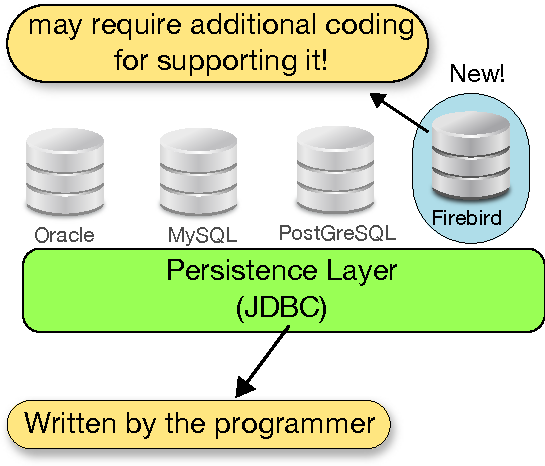
\includegraphics[keepaspectratio,width=.65\textwidth]{DB-Diversity}

Sometimes (i.e., OFTEN!) a modular and stable Pure JDBC model is hard to achieve.

\end{center}

\end{frame}


%%%%%%%%%%%%%%%%%%%%%%%%%%%%%%%%%%%%%%%%%%%%%%%%%%%%%%
%%%%%%%%%%%%%%%%%%%%%%%%%%%%%%%%%%%%%%%%%%%%%%%%%%%%%%
\section{Pure JDBC vs JPA}
\subsection{Pure JDBC Model}
\begin{frame}{\underline{Pure JDBC Model} (1)}
\justifying
%Let's open source code example of the \textbf{jdbc-persistence project}.

\begin{center}

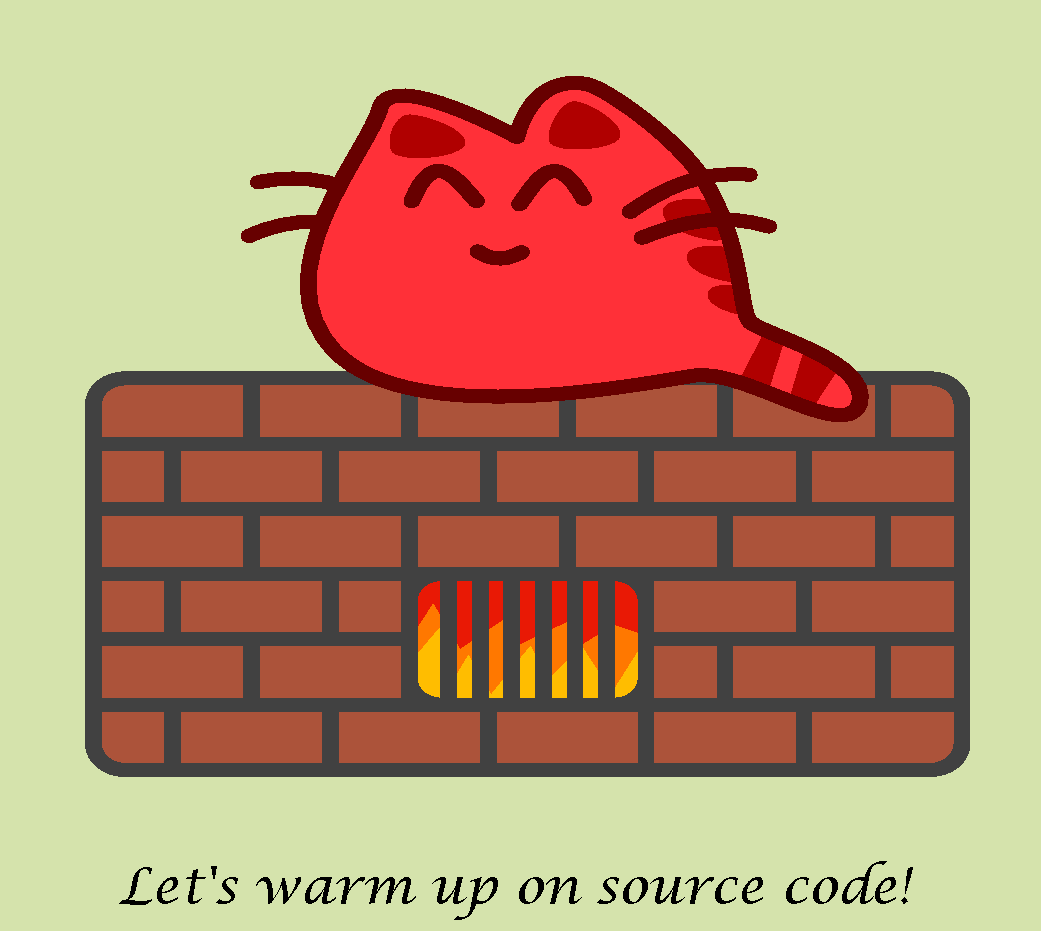
\includegraphics[keepaspectratio,width=.6\textwidth]{happycat}

\end{center}

\end{frame}

%%%%%%%%%%%%%%%%%%%%%%%%%%%%%%%%%%%%%%%%%%%%%%%%%%%%%%
%%%%%%%%%%%%%%%%%%%%%%%%%%%%%%%%%%%%%%%%%%%%%%%%%%%%%%
\subsubsection{JPA Model}
\begin{frame}{\underline{JPA Model}}
\justifying
\begin{center}
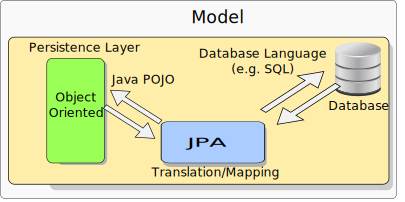
\includegraphics[keepaspectratio,width=.9\textwidth]{JPA-role}

Transparent translation and mapping of a object oriented model to different kind of storage systems.
\end{center}
\end{frame}

%%%%%%%%%%%%%%%%%%%%%%%%%%%%%%%%%%%%%%%%%%%%%%%%%%%%%%
%%%%%%%%%%%%%%%%%%%%%%%%%%%%%%%%%%%%%%%%%%%%%%%%%%%%%%
\begin{frame}{\underline{JPA Model} (1)}
\justifying

%Let's take a look on the \textbf{jpa-persistence project}.

\begin{center}

\includegraphics[keepaspectratio,width=.5\textwidth]{Happy-Tiger}


\end{center}
\end{frame}

%%%%%%%%%%%%%%%%%%%%%%%%%%%%%%%%%%%%%%%%%%%%%%%%%%%%%%
%%%%%%%%%%%%%%%%%%%%%%%%%%%%%%%%%%%%%%%%%%%%%%%%%%%%%%
\section{\scshape ORM}
\begin{frame}{\underline{Object-Relational Mapping (ORM)}}

\begin{center}
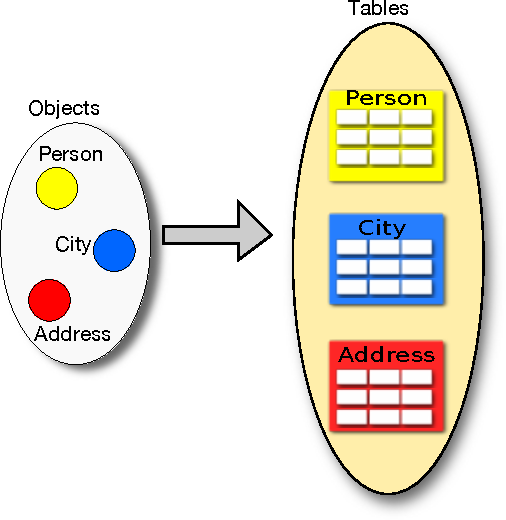
\includegraphics[keepaspectratio,width=.65\textwidth]{objectToTable}

\end{center}

\end{frame}

%%%%%%%%%%%%%%%%%%%%%%%%%%%%%%%%%%%%%%%%%%%%%%%%%%%%%%
%%%%%%%%%%%%%%%%%%%%%%%%%%%%%%%%%%%%%%%%%%%%%%%%%%%%%%
\subsection{\scshape Mapping Strategies}
\begin{frame}{\underline{Mapping Strategies}}
\justifying

\begin{itemize}
\itemsep 12pt

\item A Table Per Concrete Class;

\item A Single Table Per Class Hierarchy;

\item A Joined Subclass Strategy.

\end{itemize}
\end{frame}
%%%%%%%%%%%%%%%%%%%%%%%%%%%%%%%%%%%%%%%%%%%%%%%%%%%%%%
%%%%%%%%%%%%%%%%%%%%%%%%%%%%%%%%%%%%%%%%%%%%%%%%%%%%%%
\subsection{\scshape Mapping Strategies}
\begin{frame}{\underline{A Table per concrete class}}
\justifying

\textbf{Advantages}:

\begin{itemize}
\itemsep 12pt
\justifying
\item Direct mapping between classes defined on the Object Oriented model and Tables on a given database;

\item All properties (included those inherited from a superclass) are included as table columns.

\end{itemize}

\textbf{Drawbacks}:
\begin{itemize}
\itemsep 12pt
\justifying
\item Poor query performance when the Object Oriented model has many relations between entities;
\item A considerable number of SQL JOINS must be need to retrieve a given set of objects from database.

\end{itemize}
\end{frame}

%%%%%%%%%%%%%%%%%%%%%%%%%%%%%%%%%%%%%%%%%%%%%%%%%%%%%%
%%%%%%%%%%%%%%%%%%%%%%%%%%%%%%%%%%%%%%%%%%%%%%%%%%%%%%
\begin{frame}{\underline{A Table per class hierarchy}}
\justifying

\textbf{Advantages}:

\begin{itemize}
\itemsep 12pt
\justifying
\item Classes sharing common properties are grouped within a single table;

\item Fast queries when the purpose is to find entities which are part of the same class hierarchy.

\end{itemize}

\textbf{Drawbacks}:
\begin{itemize}
\itemsep 12pt
\justifying
\item As all subclasses are grouped on the same table, all specific fields of each subclass should be nullable; 
\item All basic validations required to guarantee model consistency on a given subclass when inserting and/or updating data must be done by the programmer.

\end{itemize}
\end{frame}

%%%%%%%%%%%%%%%%%%%%%%%%%%%%%%%%%%%%%%%%%%%%%%%%%%%%%%
%%%%%%%%%%%%%%%%%%%%%%%%%%%%%%%%%%%%%%%%%%%%%%%%%%%%%%
\begin{frame}{\underline{A Joined Subclass Strategy}}
\justifying

\textbf{Advantages}:

\begin{itemize}
\itemsep 12pt
\justifying
\item Superclass and Subclass fields are represented as separated tables.

\item Provides support for polymorphic relationships.

\end{itemize}

\textbf{Drawbacks}:
\begin{itemize}
\itemsep 12pt
\justifying
\item May require or or more SQL JOIN operations to instantiate objects from specific subclasses;
\item The performance of database access is dependent on the complexity of class hierarchy.

\end{itemize}
\end{frame}

%%%%%%%%%%%%%%%%%%%%%%%%%%%%%%%%%%%%%%%%%%%%%%%%%%%%%%
%%%%%%%%%%%%%%%%%%%%%%%%%%%%%%%%%%%%%%%%%%%%%%%%%%%%%%
\subsection{\scshape Relationship Between Entities}
\begin{frame}{\underline{Relationship Between Entities}}
\justifying

The relationship between persistent entities can be of four different types (excluding inheritance):

\begin{itemize}
\itemsep 12pt
\justifying

\item OneToOne;
\item OneToMany;
\item ManyToOne;
\item ManyToMany.

\end{itemize}

\end{frame}

%%%%%%%%%%%%%%%%%%%%%%%%%%%%%%%%%%%%%%%%%%%%%%%%%%%%%%
%%%%%%%%%%%%%%%%%%%%%%%%%%%%%%%%%%%%%%%%%%%%%%%%%%%%%%
\subsection{\scshape Association}
\begin{frame}{\underline{OneToOne}}
\justifying

\begin{center}

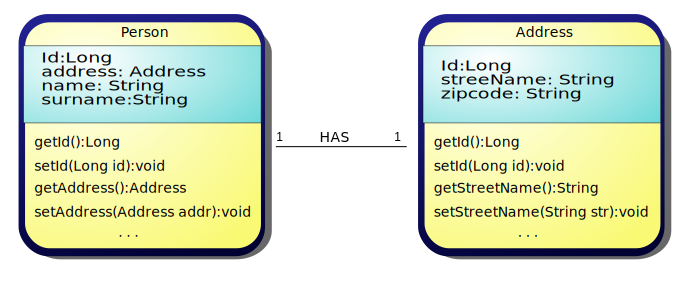
\includegraphics[keepaspectratio, width=\textwidth]{oneToOne}

\end{center}

\end{frame}

%%%%%%%%%%%%%%%%%%%%%%%%%%%%%%%%%%%%%%%%%%%%%%%%%%%%%%
%%%%%%%%%%%%%%%%%%%%%%%%%%%%%%%%%%%%%%%%%%%%%%%%%%%%%%
\begin{frame}{\underline{OneToMany}}
\justifying

\begin{center}

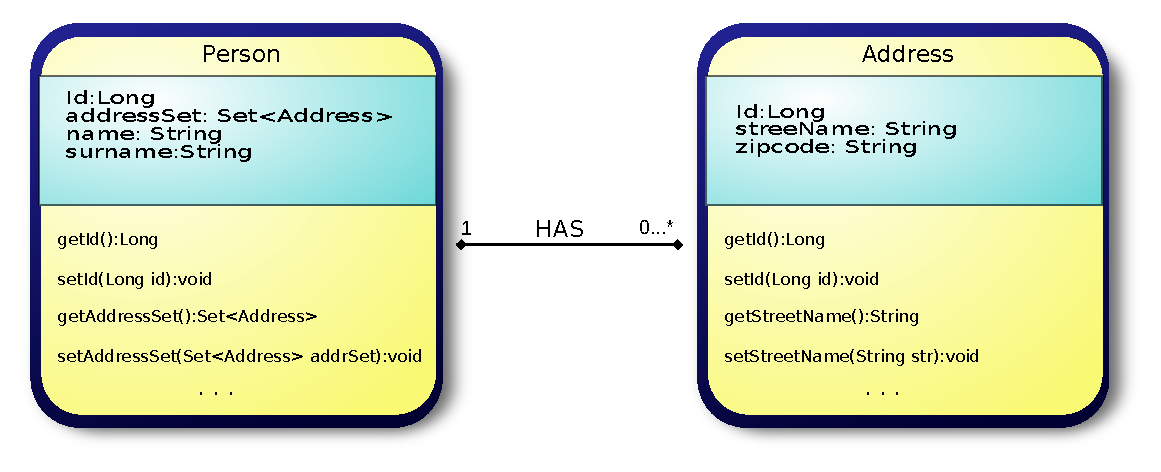
\includegraphics[keepaspectratio, width=\textwidth]{oneToMany}

\end{center}

\end{frame}

%%%%%%%%%%%%%%%%%%%%%%%%%%%%%%%%%%%%%%%%%%%%%%%%%%%%%%
%%%%%%%%%%%%%%%%%%%%%%%%%%%%%%%%%%%%%%%%%%%%%%%%%%%%%%
\begin{frame}{\underline{ManyToOne}}
\justifying

\begin{center}

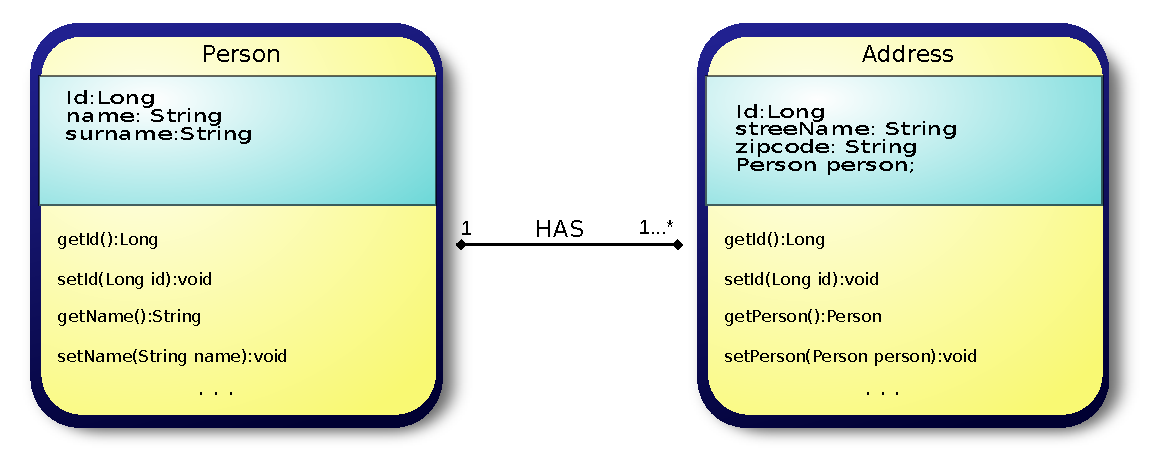
\includegraphics[keepaspectratio, width=\textwidth]{manyToOne}

\end{center}

\end{frame}

%%%%%%%%%%%%%%%%%%%%%%%%%%%%%%%%%%%%%%%%%%%%%%%%%%%%%%
%%%%%%%%%%%%%%%%%%%%%%%%%%%%%%%%%%%%%%%%%%%%%%%%%%%%%%
\begin{frame}{\underline{ManyToMany}}
\justifying

\begin{center}

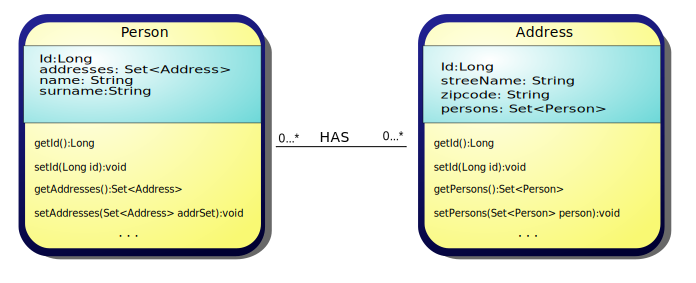
\includegraphics[keepaspectratio, width=\textwidth]{manyToMany}

\end{center}

\end{frame}

%%%%%%%%%%%%%%%%%%%%%%%%%%%%%%%%%%%%%%%%%%%%%%%%%%%%%%
%%%%%%%%%%%%%%%%%%%%%%%%%%%%%%%%%%%%%%%%%%%%%%%%%%%%%%
\section{\scshape Persistence Provider}
\begin{frame}{\underline{Persistence Provider}}
\begin{itemize}
\itemsep 12pt
\justifying

\item It is the concrete implementation of the JPA exposed interfaces;

\item As the behaviour of implementations are not defined within the Standard, different Persistence Providers may behave differently on the same set of inputs;

\item The two most utilised persistence providers are the \textit{Hibernate} and the \textit{EclipseLink}.
\end{itemize}
\end{frame}

%%%%%%%%%%%%%%%%%%%%%%%%%%%%%%%%%%%%%%%%%%%%%%%%%%%%%%
%%%%%%%%%%%%%%%%%%%%%%%%%%%%%%%%%%%%%%%%%%%%%%%%%%%%%%
\subsection{Hibernate: The Entrepreneur}
\begin{frame}{Hibernate: The Entrepreneur}

\begin{center}

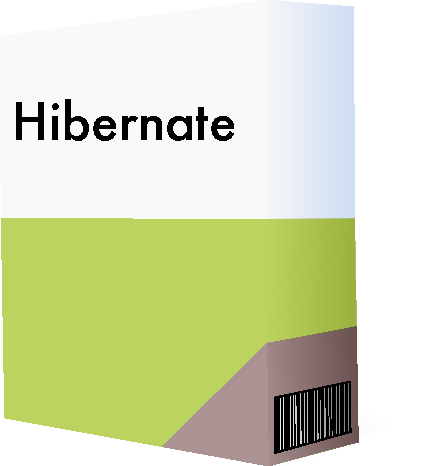
\includegraphics[keepaspectratio,width=.45\textwidth]{Hibernate}

\end{center}
\end{frame}

%%%%%%%%%%%%%%%%%%%%%%%%%%%%%%%%%%%%%%%%%%%%%%%%%%%%%%
%%%%%%%%%%%%%%%%%%%%%%%%%%%%%%%%%%%%%%%%%%%%%%%%%%%%%%
\subsection{Eclipselink: The reference implementation}
\begin{frame}{Eclipselink: The reference implementation}

\begin{center}

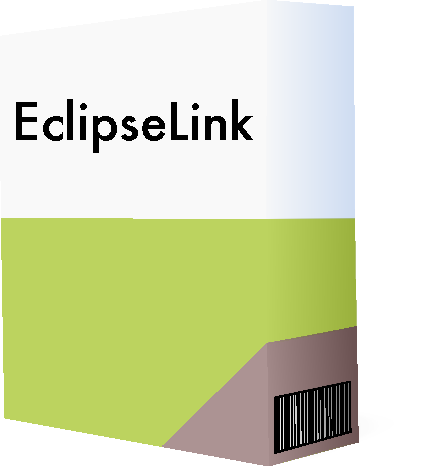
\includegraphics[keepaspectratio,width=.45\textwidth]{EclipseLink}

\end{center}
\end{frame}

%%%%%%%%%%%%%%%%%%%%%%%%%%%%%%%%%%%%%%%%%%%%%%%%%%%%%%
%%%%%%%%%%%%%%%%%%%%%%%%%%%%%%%%%%%%%%%%%%%%%%%%%%%%%%
\section{\scshape Hello World JPA}
\subsection{Example of a JPA application}
\begin{frame}{\underline{The complete Hello World JPA example}}

\begin{center}

\includegraphics[keepaspectratio,width=.4\textwidth]{Happy-Tiger-Hello}
\end{center}
\end{frame}

%%%%%%%%%%%%%%%%%%%%%%%%%%%%%%%%%%%%%%%%%%%%%%%%%%%%%%
%%%%%%%%%%%%%%%%%%%%%%%%%%%%%%%%%%%%%%%%%%%%%%%%%%%%%%
\begin{frame}[noframenumbering]{External sources}

\begin{itemize}
\itemsep 12pt
\justifying

\item JPA Specification: JSR 220 (\url{https://www.jcp.org/en/jsr/detail?id=220});

\item OpenClipart (\url{https://openclipart.org/});

\item Inkscape (\url{https://inkscape.org/en/});

\item \LaTeX $\;$Project (\url{http://www.latex-project.org/});

\item \LaTeX $\;$Beamer (\url{https://bitbucket.org/rivanvx/beamer/wiki/Home}).

\end{itemize}




\end{frame}

%%%%%%%%%%%%%%%%%%%%%%%%%%%%%%%%%%%%%%%%%%%%%%%%%%%%%%
%%%%%%%%%%%%%%%%%%%%%%%%%%%%%%%%%%%%%%%%%%%%%%%%%%%%%%
\begin{frame}[plain,noframenumbering]

\begin{center}

\includegraphics[keepaspectratio, width=.8\textwidth]{happycat-end}
\end{center}
\end{frame}

\end{document}